%\documentclass[../main.tex]{subfiles}
%\begin{document}
Process mining is a relatively new discipline that has emerged from the need to bridge the gap of data mining and business process management. The objective of process mining is to support the analysis of business processes, provide valuable insights on processes and further improve the business execution. According to \cite{van2011process}, techniques of process mining are divided into three categories: process discovery, conformance checking, and process enhancement. Process discovery techniques derive visual models from event logs of the information system, aiming at a better understanding of real business processes. Conformance checking analyzes the deviations between a referenced process model and observed behaviors driven from its execution. Enhancement adapts and improves existing process models by extending the model with additional data perspectives or repairing the existing model to accurately reflect observed behaviors. 

Most of the organizations have predefined process execution rules which are composed of the process model. However, in real life, business processes often encounter exceptional situations where it is necessary to execute process differing from the referred model. To reflect reality, the organizations need to adjust the existing process model. Basically, one can apply process discovery techniques again to obtain a new model from event log. However, due to the facts, (1) the cost of rediscovery, and (2)  the discovered model tend to have less similarity with the original model\cite{fahland2012repairing}. As shown in \cite{fahland2012repairing}, there is a need to change an existing model similar to the original model while replaying the current process execution. Here comes the model repair. 

Model repair belongs to process enhancement\cite{fahland2012repairing}. It analyzes the workflow deviations between an event log and a process model, and fix the deviations mainly by adding subprocesses on the model. As known, business in organizations is goal-oriented and aims to have high performance according to a set of Key Performance Indicator(KPI)s,e.g. average conversion time for the sales, payment error rate for the finance.  However, little research in process mining is conducted on the base of business performance\cite{ghasemi2019event}.  \cite{ghasemi2019event} points out several contributions like \cite{dees2017enhancing} to consider business performance into process mining. The work in \cite{dees2017enhancing} divides deviations of model and the event log into positive and negative with certain KPIs. Then it applies repair techniques in \cite{fahland2015model} only with positive deviations, to avoid introducing negative instances into the repaired model. 

However, the current repair methods have some limits. Model repair techniques fix the model by adding subprocesses. They guarantee the model fitness but overgeneralizes the model, such that it allows more behaviors than expected. On the other hand, it increases the model complexity.  Even the performance is considered in \cite{dees2017enhancing}, but only deviations in positive is used to add subprocesses, the negative information is ignored, which disables the possibility to block negative behaviors from model.  A motivation example is listed to describe those limits.
%% Motivation 
\section{Motivation Example}
\begin{wrapfigure}{r}{0.3\textwidth}
	\centering
	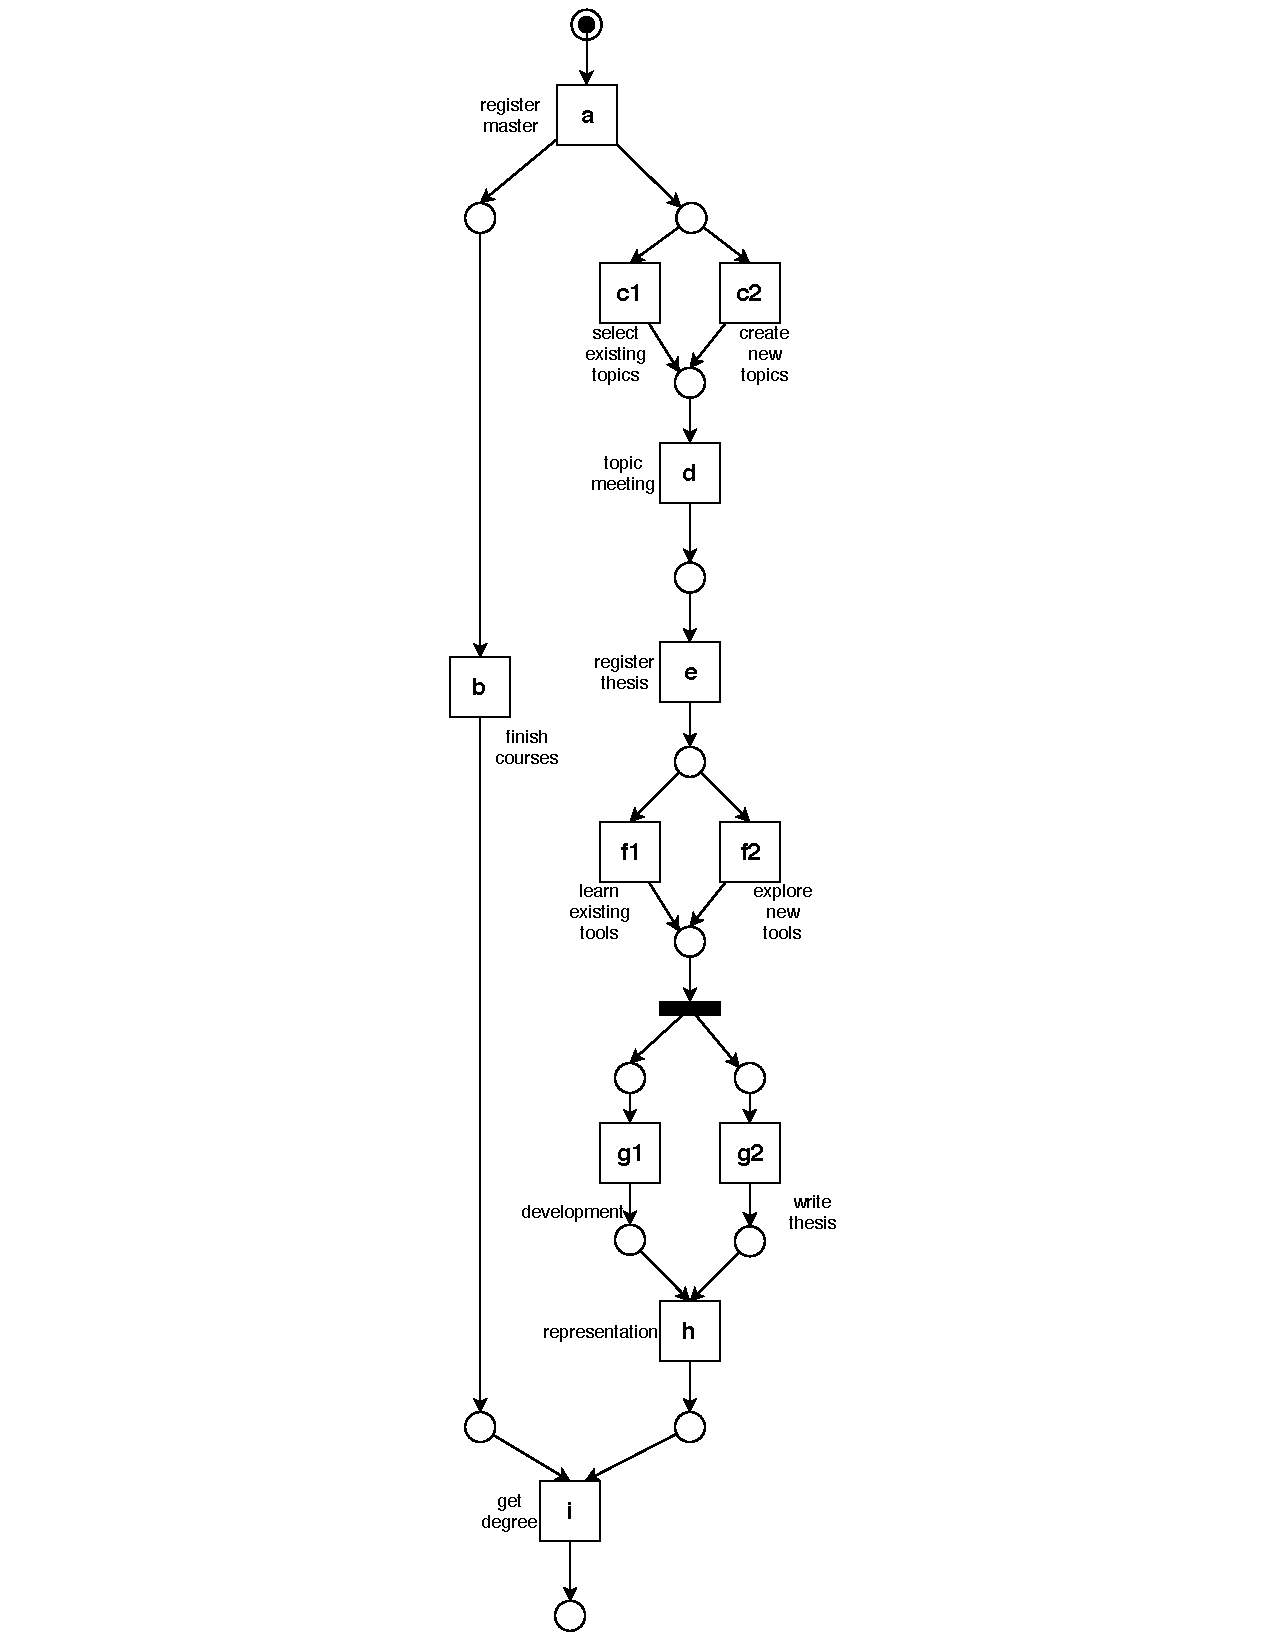
\includegraphics[clip, trim=7cm 0cm 7cm 0cm, width=0.4\textwidth, height=0.7\textheight]{figures/introduction/Master-original-model.pdf}
	\caption{original master study process $M_0$}
	\label{fig:model_M0}
\end{wrapfigure}
% In this section, we use thesis registration example to display the shortcomings of existing techniques and then introduces our methods, but we need to answer them later..
This section describes some situations where current repair techniques can't handle properly. For the sake of understanding, examples are extracted from the common master study procedure to illustrate those situations.

The main activities for the master study include \emph{register master}, \emph{finish courses} and \emph{write a master thesis}. Here, we simplify the \emph{finish courses} and only extend the activity \emph{write a master thesis} into a set of sub activities as our examples. Those activities are shown in the Petri net model $M_0$ of Figure \ref{fig:model_M0}. The activities are modeled by the corresponding \textbf{\emph{transitions}} which is represented by a square. Transitions are connected through a circle called \textbf{\emph{place}}. Transitions and places build the static structure of Petri net and describe the transition relations. \textbf{\emph{Tokens}} in the black dot are put in the initial places and represent the dynamic state of the model. 

$M_0$ is currently in an initial state where only one token is at the start place to enable the transition \emph{register master}. After firing \emph{register master}, the token at the initial place is consumed while two new token are generated in the output places of \emph{register master}. In this way, activity \emph{finish courses}  can be executed in concurrence with the other branch except for the \emph{get degree}. When multiple activities have the same input place, all of them are enabled but only one of them can be fired and executed, namely, they are exclusive to each other. As shown in the figure,  \emph{select existing topics}  and \emph{create new topics} are exclusive, and only one of them can be triggered. When a transition has multiple input places, it can be triggered with condition that all input places hold at least a token. \emph{Get degree} is enabled only after \emph{finish courses} and \emph{representation} done. 


% here we are going to talk about the situations where the current repair method can not handle well.
%talk about the execution trace definition. 
Along the tokens flowing through the model, activities get fired and institute a sequence according to their execution order. One execution sequence is called one trace. A set of traces depicts the model behavior and is recorded into a data file called event log. With the running of process model in real life, activities can be executed with difference to the model. A trace which has no deviation to the model is fit. Otherwise, it's a unfit trace. With accumulation of deviations, process model needs amending to reflect reality.  In the following part, different several situations are introduced to demonstrate the shortcomings of current techniques to repair a model. 
\subsection{Situation 1: \small{repair model with unfit traces}} % add preparation to this model
In some universities, before registering a master thesis, activities \emph{write proposal} and \emph{check course requirement} with exclusive relation might be necessary. Their real master study procedures are recorded in the event log $L_1$. Traces with either of those activities are considered as positive. For convenience, alphabet characters are used to represent the corresponding activities and annotated in the model. \textbf{x1, x2} represent the activities \emph{write proposal} and \emph{check course requirement}.
\emph{Event Log $L_1$ -- }
		\begin{align*}
		Positive:\{ & { <a,b, c1,d,\textbf{e1},f,g1,g2,h,i>}^{50}, \\   &{<a,b, c2,d,\textbf{e2},f,g2,g1,h,i>}^{50} \}
		% Negative: \{ & {<a,c1,d,\quad f,g1,h>}^{50} \}
		\end{align*}
\begin{figure}[htp]
	\centering
	\begin{subfigure}[b]{0.5\textwidth}
		\centering
		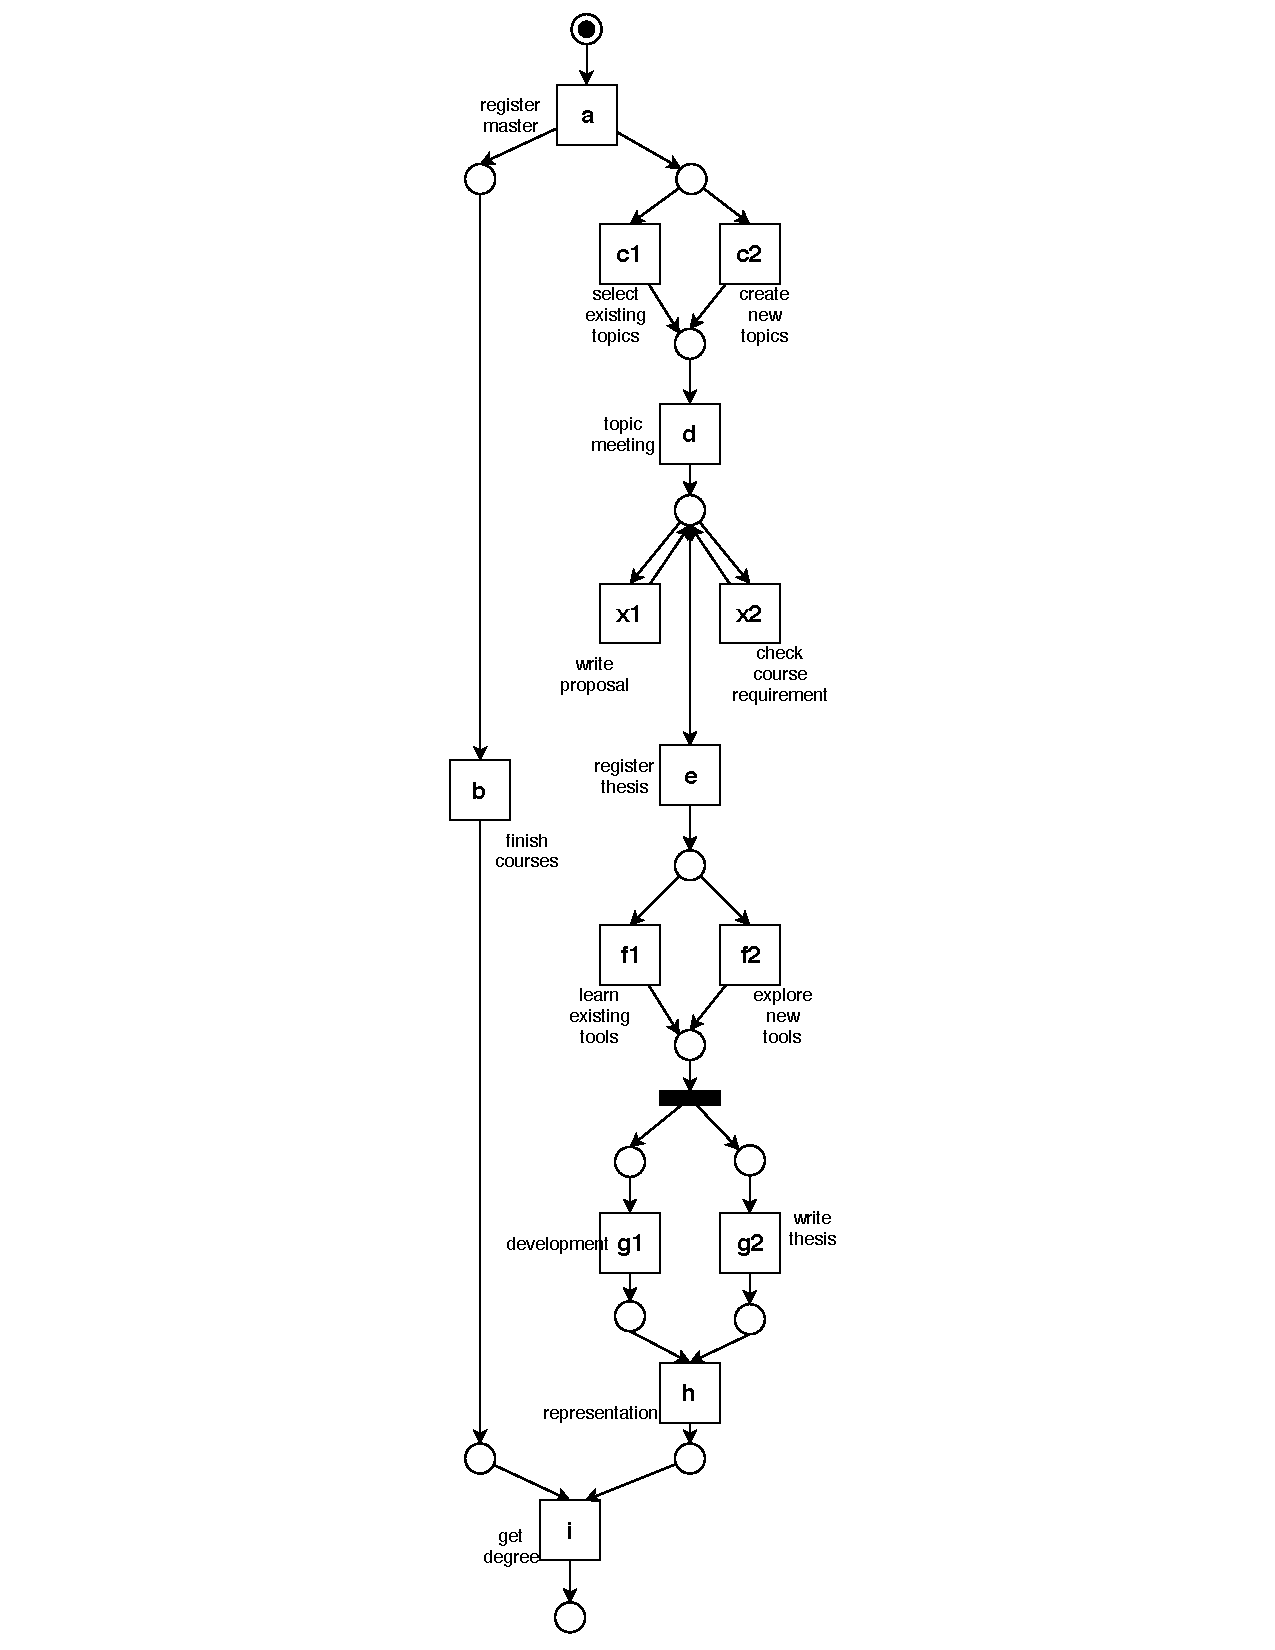
\includegraphics[clip, trim=7cm 0cm 7cm 0cm, width=0.5\linewidth, height=0.7\textheight]{figures/introduction/Master-add-events-loop.pdf}
		\caption{repaired model $M_{1.1}$ with additional activities }
		\label{fig:model_b1}
	\end{subfigure}%
	\begin{subfigure}[b]{0.5\textwidth}
		\centering
		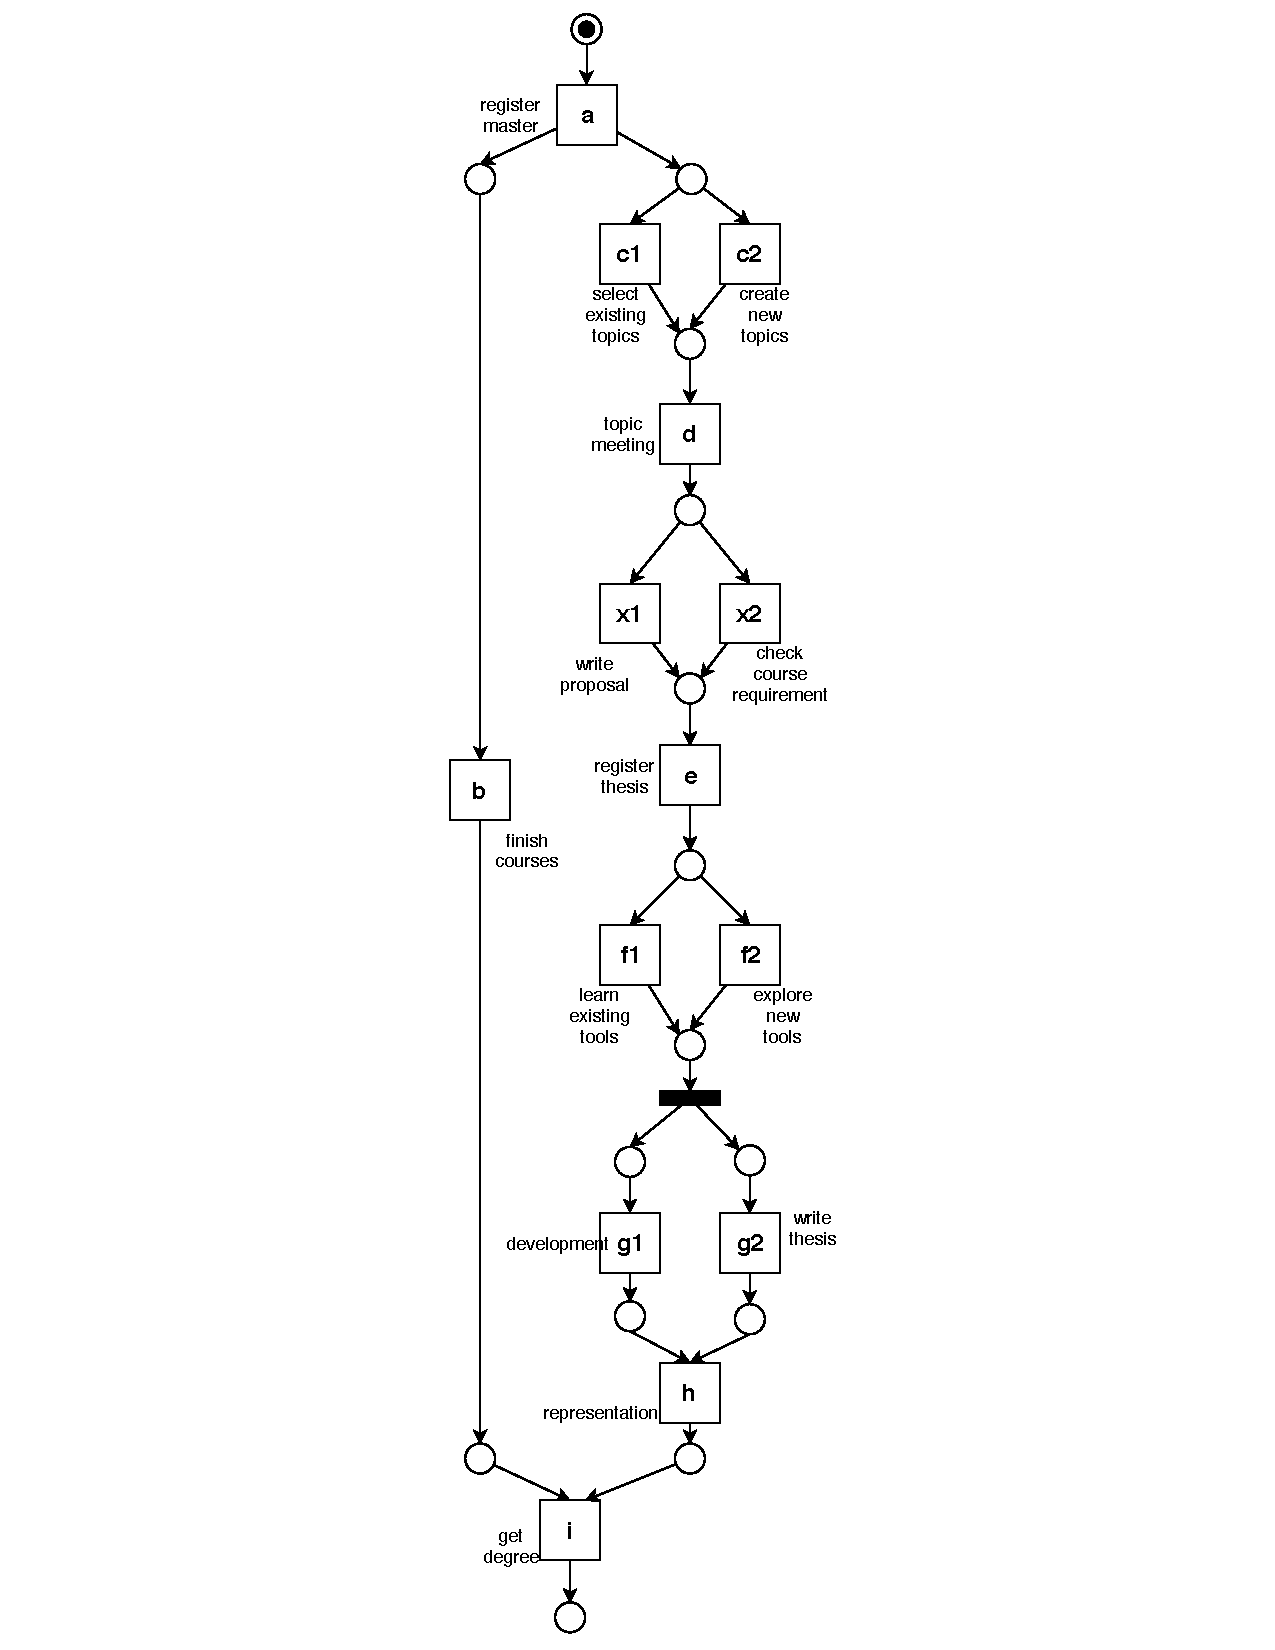
\includegraphics[clip, trim=7cm 0cm 7cm 0cm, width=0.5\linewidth, height=0.7\textheight]{figures/introduction/Master-add-events.pdf}
		\caption{expected model $M_{1.2}$ with additional activities}
		\label{fig:model_b2}
	\end{subfigure}
	\caption{example for situation 1}
	\label{fig:model_change_1}
\end{figure}

Because the repair techniques in \cite{fahland2015model} don't distinguish the performance of event log, all instances with positive labels are employed to repair the model. Firstly, the deviations of the existing model in Figure \ref{fig:model_a} and the event log $L_1$ is computed. After computation of deviations, each deviation has the same start and end place and two deviations appear at the same position in the model. When repairing this model, each subprocess has one place as its start and end place, which forms a loop in the model. If there is only one such subprocess, the subprocess will be added in a sequence in the model, which leads to a higher precision. Yet the algorithm does not discover orderings between different subprocesses at overlapping locations. So subprocesses are kept in a loop form. 

The repaired model is shown in Figure \ref{fig:model_b1}, where the two additional activities are added in the form of loop. The repair algorithm in \cite{dees2017enhancing} builds upon \cite{fahland2015model} and considers the performance of the event log. However, the repaired model is the same as the one in Figure \ref{fig:model_b1}. The reasons are: (1) there is no deviation from negative factors. (2) positive deviations are used in the same way as \cite{fahland2015model}. 

Compared to the model in Figure \ref{fig:model_b1} where the two extra activities are shown in loop, the model in Figure \ref{fig:model_b2} are more expected, since it includes the two activities in sequence and has a higher precision.

\subsection{Situation 2: \small{repair model with fit traces}}
% we should delete the prepare carefully and casually from the model. Only consider to add the data about the order change..what we expect is not 
This situation describes the existing problem in the current methods that fit traces with negative performance outcomes cannot be used to repair a model. Given an actual event log $L_2$, when activity \emph{finish courses} is fired after \emph{begin thesis} and before writing master thesis, it reduces the pressure for the master thesis phase and traces in such an order are treated as positive. Else, the negative outcomes are given. 
\emph{Event Log $L_2$ -- }
\begin{align*}
Positive:\{ & { <a,\textbf{b},c1,d,f,g2,g1,h,i>}^{50}, \\   &{<a,\textbf{b},c2,d,f,g1,g2,h>}^{50} \}  \\
Negative: \{ & {<a,c1,d,f,g2,g1,\textbf{b},h,i>}^{50}, \\
& {<a,c1,\textbf{b},d,f,g1,g2,h,i>}^{50},  \}
\end{align*}
Compared to the model, the event log $L_2$ contains no deviation. When we apply the techniques in \cite{fahland2015model} and \cite{dees2017enhancing} to repair the model, the model keeps untouched due to no deviation. Apparently, the reason that those two methods can't incorporate the negative information in fit traces causes this shortcoming. When we expect a model which enforce the positive instances and avoid the negative instance as the model $M_2$, the current methods fail our need. 
\begin{figure}[htp]
	\centering
	\begin{subfigure}[b]{0.5\textwidth}
		\centering
		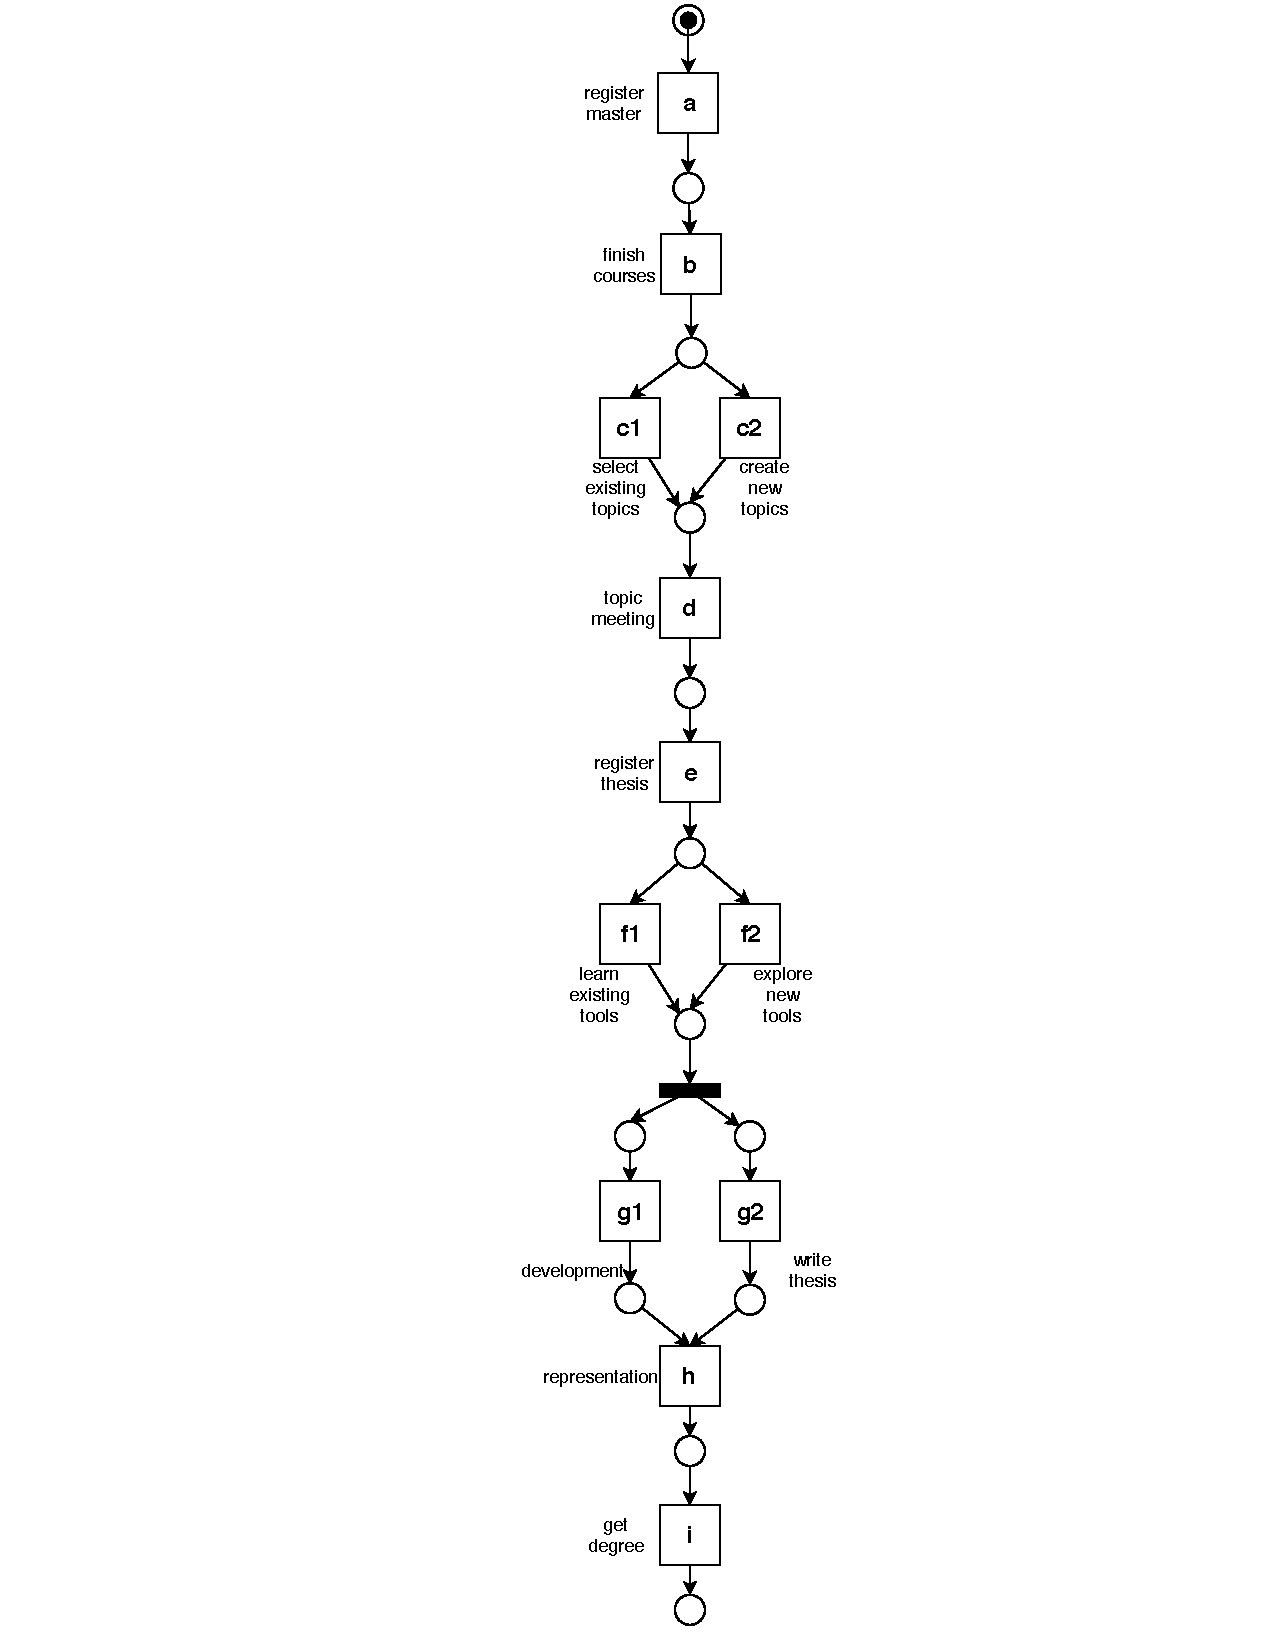
\includegraphics[clip, trim=8cm 0cm 8cm 0cm, width=0.5\linewidth, height=0.7\textheight]{figures/introduction/Master-change-order.pdf}
		\caption{expected model $M_{2}$ with order change}
		\label{fig:model_c}
	\end{subfigure}%
	\begin{subfigure}[b]{0.5\textwidth}
		\centering
		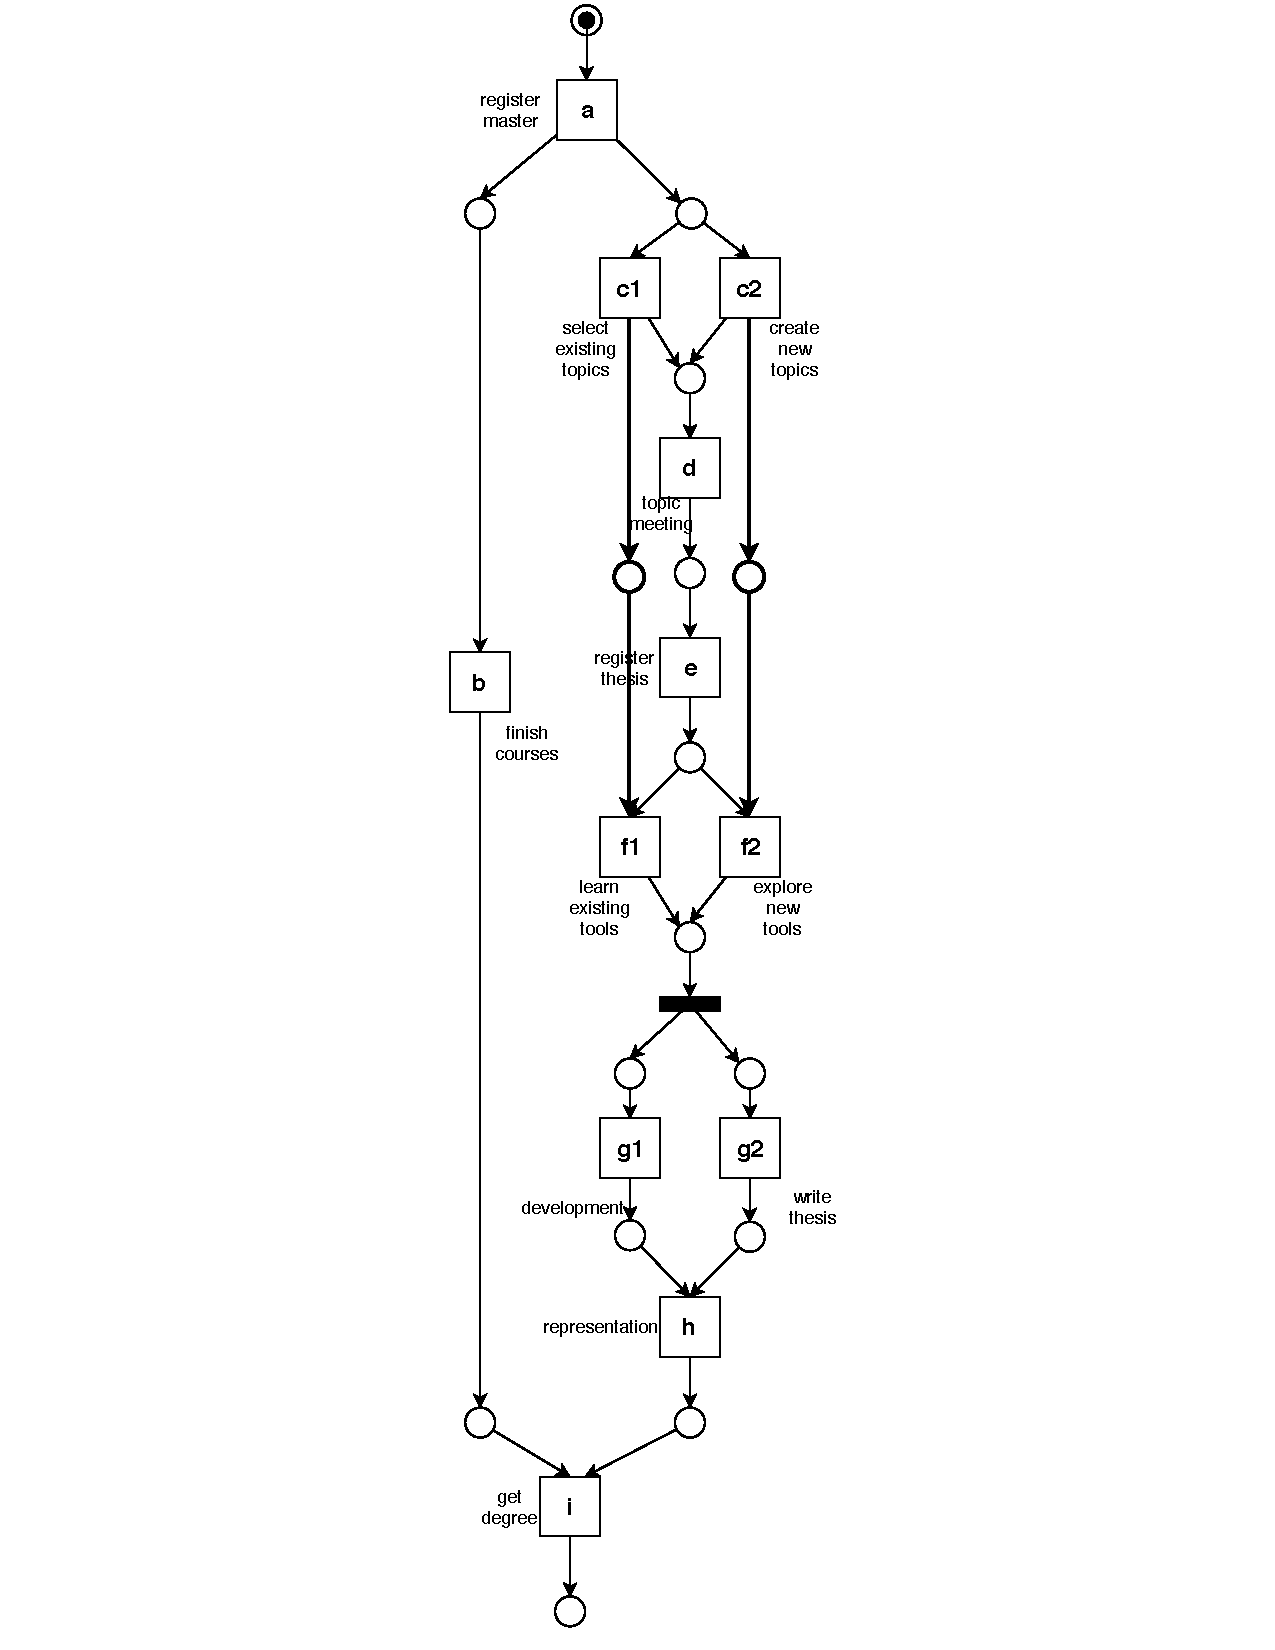
\includegraphics[clip, trim=7cm 0cm 7cm 0cm, width=0.5\linewidth, height=0.7\textheight]{figures/introduction/Master-with-lt.pdf}
		\caption{model $M_{3}$ with long-term dependency}
		\label{fig:model_d}
	\end{subfigure}
	\caption{example for situation 2 and 3}
	\label{fig:model_changes_2_3}
\end{figure}
\subsection{Situation 3: \small{detect long-term dependency}}
This part introduces a problem which causes a lower precision in process mining. It is the inability in current methods to detect the long-term dependency in the Petri net. The long-term dependency describes the phenomenon that one execution choice decides the execution of activities that do not follow directly. Due to the long distance of this dependency, current methods cannot detect it and improve the precision by adding long-term dependency on the model. 
An event log $L_3$ is given in the following. By using time consumption as one KPI, if the total sum goes over one threshold, we mark this trace as negative, else as positive. Since the activity \emph{create new topics} usually demands new knowledge rather than checking the existing tools. So if students choose to learn existing tools, it's possibly not useful and time is wasted. In the other case, if we select existing topics with existing background, it saves time when we directly learn the existing tools. According to this performance standard, we classified those event traces.
\emph{Event Log $L_3$ -- }
\begin{align*}
Positive:\{ & { <a,b,\textbf{c1},d,e,\textbf{f1},g1,g2, h,i>}^{50}, \\   &{<a,b,\textbf{c2},d,e,\textbf{f2},g2,g1, h,i>}^{50} \}  \\
Negative: \{ & {<a,b,\textbf{c1},d,e,\textbf{f2},g2,g1,h,i>}^{50}, \\
& {<a,b,\textbf{c2},d,e,\textbf{f1},g1,g2,h,i>}^{50}  \}
\end{align*}
%here we list one example to explain the long-term dependency, but we need to make them clear, might without the loop item..It means that we need to change the whole model..
There are no deviations of the model and event log $L_3$ according to the  algorithms in \cite{fahland2015model} and \cite{dees2017enhancing}. Therefore, the original model stays the same and allows for the execution of negative instances. After checking the model and log, those long-term dependencies have significant evidence. Transition \textbf{\emph{c1}} decides \textbf{\emph{f1}} while \textbf{\emph{c2}} decides \textbf{\emph{f2}}.  After addressing long-term dependency like the model $M_3$ in Figure \ref{fig:model_d} by connecting transitions to extra places, 
negative instances are blocked and the model has higher precision.

Clearly, the use of negative information can bring significant benefits, e.g, enable a controlled generalization of a process model: the patterns to generalize should never include negative instances. The demand to improve current repair model techniques with incorporating negative instances appears. In the next section, the demand is analyzed and defined in a formal way.

\section{Research Problem And Questions}
After analyzing the current model repair methods, we give the formal definition on the research problem of this thesis.
\begin{definition}
Given an input of one existing process model M, an event log L with performance outcomes, how to improve current process enhancement techniques by incorporating negative information, and generate a process model to enforce the positive instances while blocking the negative instance, with condition that the generated model should be as similar to the original model as possible Therefore, the repaired model provides a better way to understand and execute the real business process compared to the original model.
\end{definition}
\begin{figure}
	\centering
	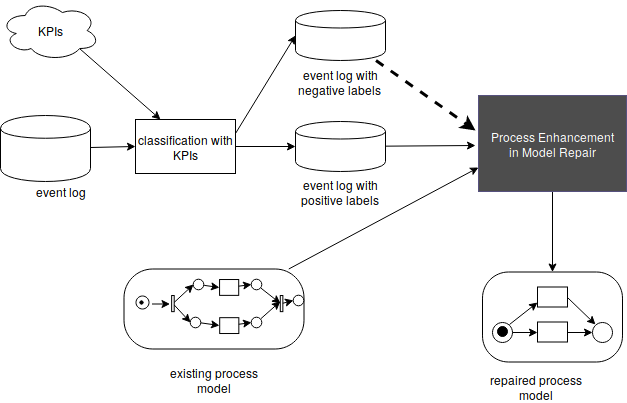
\includegraphics[width=\textwidth]{figures/introduction/FD_approach_blackbox.png}
	\caption{The problem description}
	\label{fig:method_architecture}
\end{figure}
An event log and an existing model are given as the input shown in Figure \ref{fig:method_architecture}. According to predefined KPIs, each trace in event log is classified into positive or negative. After applying repair techniques in the black box, the model should be improved to enforce the positive instances while disallowing negative instance.  

To solve this research problem, the following questions should be answered. 
\begin{itemize}
	\item How to balance the impact of the existing model, negative and positive instances together to repair model? 
	\item How to block negative instances from the model while enforcing the positive ones?
	\item Does this method overcome the shortcomings of other repair techniques? 
\end{itemize}


To answer those questions, we propose a solution in this paper. It analyzes process performance on trace level and balances the existing model, positive traces and negative traces on directly-follows relation, in order to incorporate all the factors on model generation. Experiments are conducted to answer the questions.  
Later, the directly-follows relation is used to create process model by Inductive Miner. 


\section{Outline}
This thesis tries to answer the questions above in the remainder sections and provide a solution for the black box. 

Section 2 and 3 introduces the related work and recalls the basic notions on process mining and list the preliminary to solve the problem. 

The next section answers the questions, how to balance all factors and block negative instances, Our algorithm analyzes process performance on trace level and balances the existing model, positive traces and negative traces on directly-follows relation, in order to incorporate all the factors on model generation. Long-term dependency is further detected on the intermediate model and added to block negative instances. What's more, the impact of the existing model, positive and negative instances are parameterized by weights, to allow more flexibility of the generated model.

In Implementation Section, screenshots are given from the finished tools of our algorithm to demonstrate the use. 

Experiment section answers the last question, if our method overcomes the existing shortcomings of current repair techniques. A bundle of experiments are conducted and later results are analyzed and discussed. 

At last, we summary our work in conclusion part. 

%\end{document}